\section{Stripe}
\label{sec:stripe}
Stripe is an Irish technology company that allows both private individuals and businesses to accept payments over the Internet \cite{stripe_doc_a}.
Stripe aims to expand internet commerce by making it easy to process transactions and manage an online business.
\begin{figure}[htb]
\centering

\includegraphics[width=0.5\linewidth]{images/chapter2/stripe-logo.png}\hfill
\caption[Stripe logo]{Stripe logo}
\label{fig:stripe_logo}
\end{figure}
Stripe is 365 people and headquartered in an old trunk factory in the Mission district of San Francisco. The company has received around \$300 million in funding to date; investors include Sequoia Capital, Visa, American Express, Peter Thiel, and Elon Musk. Stripe enables you to accept payments in minutes. Collect your customers’ payment information easily and securely on web or mobile, and create charges server-side. Stripe supports 100+ currencies out of the box. In addition to credit and debit cards, Apple Pay, Android Pay, you can also easily support Bitcoin, Alipay, or Amex Express Checkout.
\newline
Stripe is a new widely celebrated alternative to Paypal and other payment gateways. Here are the main benefits of using the Stripe extension:
\begin{itemize}
\item Accept credit cards: process credit card orders directly on your site;
\item Increase sales: seamless checkout experience within your own site means increased conversions and/or sales;
\item Lower fees: competitive pricing (in many cases cheaper) than Paypal and other gateways;
\item Advanced analytics \& reporting – Beautiful analytics dashboard and sales reporting in Stipe.com;
\item PCI compliance: keeps your customers’ data safe on Stripe’s PCI compliant servers;
\item Incredibly simply setup and configuration. Buyers never leave your site to make the purchase;
\item No hidden fees: don’t get charged for refunds or disputes;
\item Global: business in any of these countries can accept payments from customers anywhere in the world;
\end{itemize}
\subsection{How it works}
Even Stripe, as Braintree, provides a default widget that you can use to integrate payments.
\begin{figure}[htb]
  \centering
  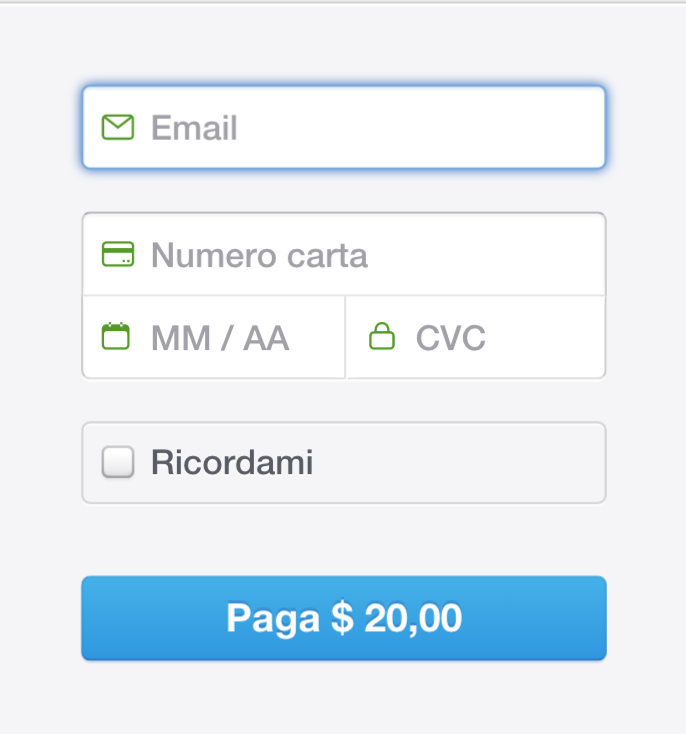
\includegraphics[width=0.5\linewidth]{images/chapter2/stripe-drop.png}\hfill
  \caption[Default stripe payment widget]{Default stripe payment widget}
\label{fig:stripe_default_ui}
\end{figure}
To get this widget, just enter the following code in its page:
\begin{lstlisting}[language=html]
<form action="" method="POST">
  <script
    src="https://checkout.stripe.com/checkout.js" class="stripe-button"
    data-key="pk_test_6pRNASCoBOKtIshFeQd4XMUh"
    data-amount="2000"
    data-name="Demo Site"
    data-description="2 widgets ($20.00)"
    data-image="/128x128.png"
    data-locale="auto">
  </script>
</form>
\end{lstlisting}
The most important thing to notice is the data-key attribute added to the script tag. This key identifies your account when communicating with Stripe.
\newline
Stripe also offers the ability to customize the payment form. This and other details can be discussed in Chapter 5.